\documentclass{beamer}
\mode<presentation>{
  \usetheme{Boadilla}
  \usefonttheme[onlylarge]{structurebold}
  \usefonttheme[stillsansseriflarge]{serif}
  \setbeamerfont*{frametitle}{size=\normalsize,series=\bfseries}
  % \setbeamertemplate{navigation symbols}{}
  \setbeamercovered{transparent}
}
\usepackage[english]{babel}
\usepackage[latin1]{inputenc}
\usepackage{times}
\usepackage[T1]{fontenc}
\usepackage{amsmath}
\usepackage{amssymb}
\usepackage{esint}
\usepackage{hyperref}
\usepackage{tikz}
\usepackage{xkeyval}
\usepackage{xargs}
\usepackage{verbatim}
\usepackage{listings}
\usepackage{multimedia}
\usetikzlibrary{
  arrows,
  calc,
  decorations.pathmorphing,
  decorations.pathreplacing,
  decorations.markings,
  fadings,
  positioning,
  shapes
}

\mode<handout>{
  \usepackage{pgfpages}
  \pgfpagesuselayout{4 on 1}[a4paper,landscape,border shrink=5mm]
  \setbeamercolor{background canvas}{bg=black!10}
}

\newcommand\pgfmathsinandcos[3]{%
  \pgfmathsetmacro#1{sin(#3)}%
  \pgfmathsetmacro#2{cos(#3)}%
}
\newcommand\LongitudePlane[3][current plane]{%
  \pgfmathsinandcos\sinEl\cosEl{#2} % elevation
  \pgfmathsinandcos\sint\cost{#3} % azimuth
  \tikzset{#1/.estyle={cm={\cost,\sint*\sinEl,0,\cosEl,(0,0)}}}
}
\newcommand\LatitudePlane[3][current plane]{%
  \pgfmathsinandcos\sinEl\cosEl{#2} % elevation
  \pgfmathsinandcos\sint\cost{#3} % latitude
  \pgfmathsetmacro\yshift{\cosEl*\sint}
  \tikzset{#1/.estyle={cm={\cost,0,0,\cost*\sinEl,(0,\yshift)}}} %
}
\newcommand\DrawLongitudeCircle[2][1]{
  \LongitudePlane{\angEl}{#2}
  \tikzset{current plane/.prefix style={scale=#1}}
  % angle of "visibility"
  \pgfmathsetmacro\angVis{atan(sin(#2)*cos(\angEl)/sin(\angEl))} %
  \draw[current plane] (\angVis:1) arc (\angVis:\angVis+180:1);
  \draw[current plane,dashed] (\angVis-180:1) arc (\angVis-180:\angVis:1);
}
\newcommand\DrawLatitudeCircleArrow[2][1]{
  \LatitudePlane{\angEl}{#2}
  \tikzset{current plane/.prefix style={scale=#1}}
  \pgfmathsetmacro\sinVis{sin(#2)/cos(#2)*sin(\angEl)/cos(\angEl)}
  % angle of "visibility"
  \pgfmathsetmacro\angVis{asin(min(1,max(\sinVis,-1)))}
  \draw[current plane,decoration={markings, mark=at position 0.6 with {\arrow{<}}},postaction={decorate},line width=.6mm] (\angVis:1) arc (\angVis:-\angVis-180:1);
  \draw[current plane,dashed,line width=.6mm] (180-\angVis:1) arc (180-\angVis:\angVis:1);
}
\newcommand\DrawLatitudeCircle[2][1]{
  \LatitudePlane{\angEl}{#2}
  \tikzset{current plane/.prefix style={scale=#1}}
  \pgfmathsetmacro\sinVis{sin(#2)/cos(#2)*sin(\angEl)/cos(\angEl)}
  % angle of "visibility"
  \pgfmathsetmacro\angVis{asin(min(1,max(\sinVis,-1)))}
  \draw[current plane] (\angVis:1) arc (\angVis:-\angVis-180:1);
  \draw[current plane,dashed] (180-\angVis:1) arc (180-\angVis:\angVis:1);
}
\newcommand\coil[1]{
  {\rh * cos(\t * pi r)}, {\apart * (2 * #1 + \t) + \rv * sin(\t * pi r)}
}
\makeatletter
\define@key{DrawFromCenter}{style}[{->}]{
  \tikzset{DrawFromCenterPlane/.style={#1}}
}
\define@key{DrawFromCenter}{r}[1]{
  \def\@R{#1}
}
\define@key{DrawFromCenter}{center}[(0, 0)]{
  \def\@Center{#1}
}
\define@key{DrawFromCenter}{theta}[0]{
  \def\@Theta{#1}
}
\define@key{DrawFromCenter}{phi}[0]{
  \def\@Phi{#1}
}
\presetkeys{DrawFromCenter}{style, r, center, theta, phi}{}
\newcommand*\DrawFromCenter[1][]{
  \setkeys{DrawFromCenter}{#1}{
    \pgfmathsinandcos\sint\cost{\@Theta}
    \pgfmathsinandcos\sinp\cosp{\@Phi}
    \pgfmathsinandcos\sinA\cosA{\angEl}
    \pgfmathsetmacro\DX{\@R*\cost*\cosp}
    \pgfmathsetmacro\DY{\@R*(\cost*\sinp*\sinA+\sint*\cosA)}
    \draw[DrawFromCenterPlane] \@Center -- ++(\DX, \DY);
  }
}
\newcommand*\DrawFromCenterText[2][]{
  \setkeys{DrawFromCenter}{#1}{
    \pgfmathsinandcos\sint\cost{\@Theta}
    \pgfmathsinandcos\sinp\cosp{\@Phi}
    \pgfmathsinandcos\sinA\cosA{\angEl}
    \pgfmathsetmacro\DX{\@R*\cost*\cosp}
    \pgfmathsetmacro\DY{\@R*(\cost*\sinp*\sinA+\sint*\cosA)}
    \draw[DrawFromCenterPlane] \@Center -- ++(\DX, \DY) node {#2};
  }
}
\makeatother

% not mandatory, but I though it was better to set it blank
\setbeamertemplate{headline}{}
\def\beamer@entrycode{\vspace{-\headheight}}

\tikzstyle{snakearrow} = [decorate, decoration={pre length=0.2cm,
  post length=0.2cm, snake, amplitude=.4mm,
  segment length=2mm},thick, ->]

%% document-wide tikz options and styles

\tikzset{%
  % >=latex, % option for nice arrows
  inner sep=0pt,%
  outer sep=2pt,%
  mark coordinate/.style={inner sep=0pt,outer sep=0pt,minimum size=3pt,
    fill=black,circle}%
}
\tikzset{
  % Define standard arrow tip
  >=stealth',
  % Define style for boxes
  punkt/.style={
    rectangle,
    rounded corners,
    draw=black, very thick,
    text width=8em,
    minimum height=2.5em,
    text centered},
}
\makeatletter
\newbox\@backgroundblock
\newenvironment{backgroundblock}[2]{%
  \global\setbox\@backgroundblock=\vbox\bgroup%
  \unvbox\@backgroundblock%
  \vbox to0pt\bgroup\vskip#2\hbox to0pt\bgroup\hskip#1\relax%
}{\egroup\egroup\egroup}
\addtobeamertemplate{background}{\box\@backgroundblock}{}
\makeatother

% \def\timeleft{15:00->14:55}

\title[Na update]{NaCs lab update}
\date{March 24, 2017}
\author{Yichao Yu}
\institute{Ni Group/Harvard}

\begin{document}

\begin{frame}{}
  \titlepage
\end{frame}

% \begin{frame}{}
%   \tableofcontents
% \end{frame}

\begin{frame}{}
  \begin{center}
    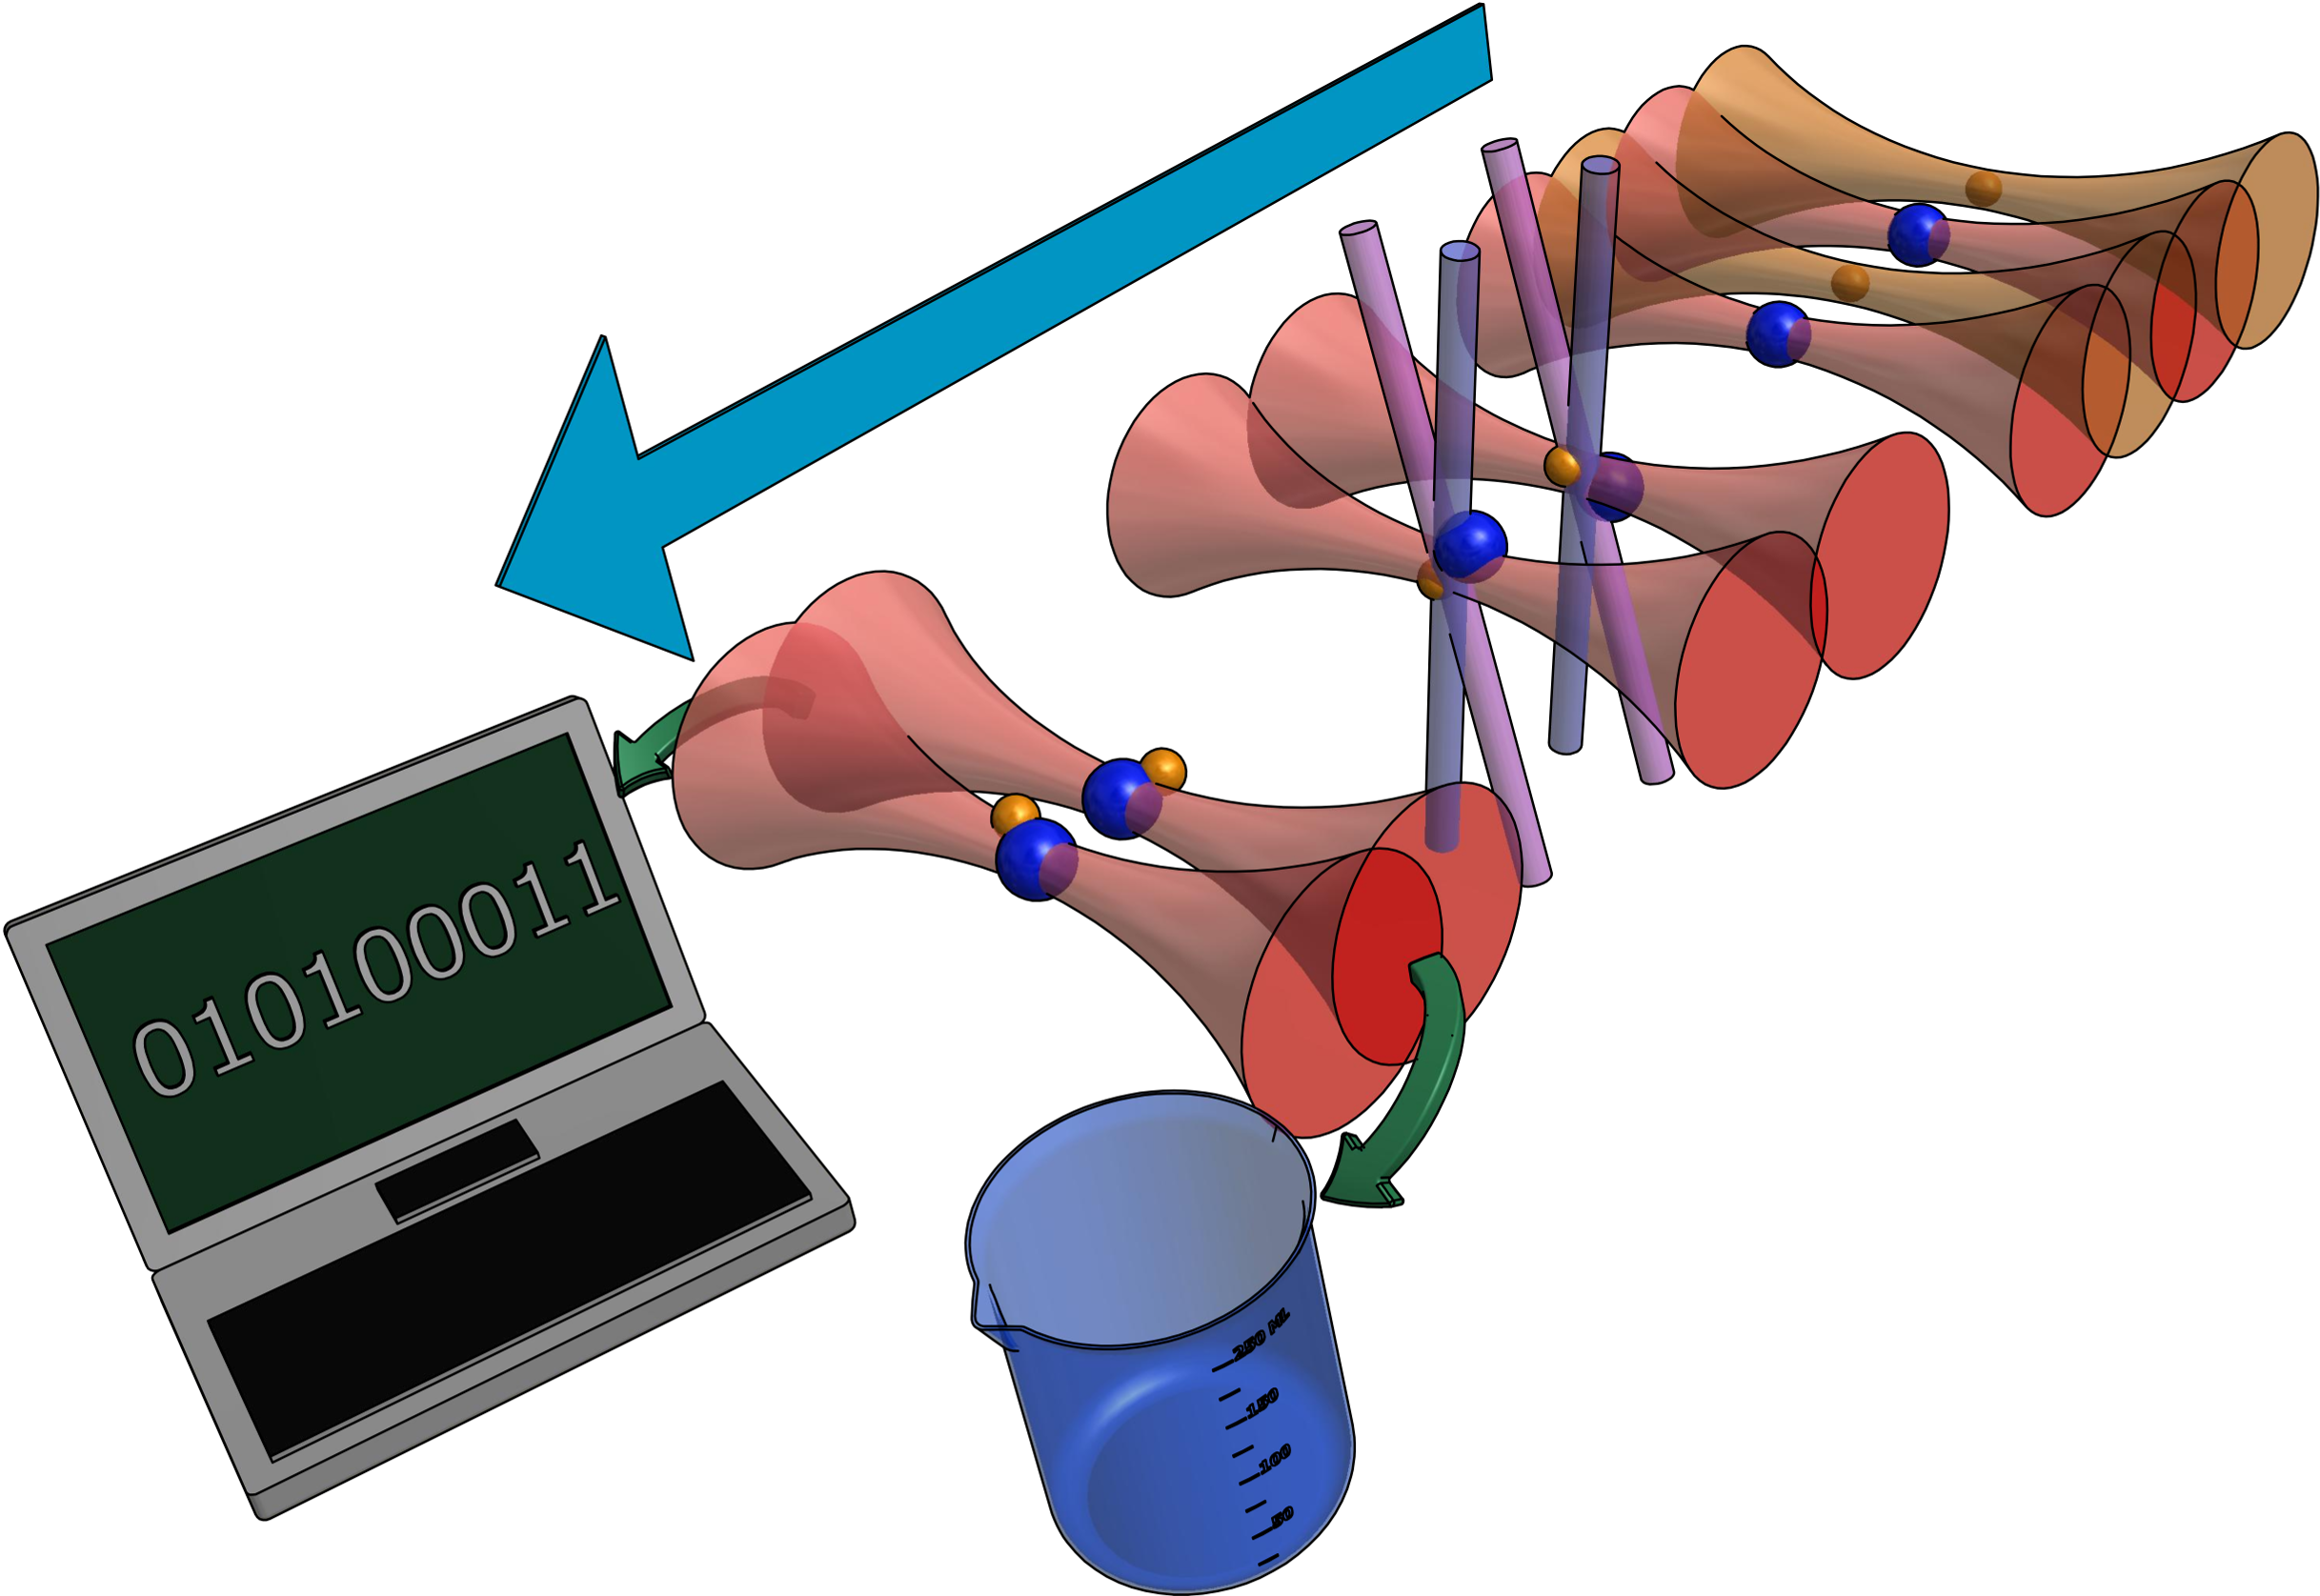
\includegraphics[width=10cm]{../damop-2016/overall_full_min.png}
  \end{center}
\end{frame}

% Axial result
% Radial result
% 3D result

\begin{frame}{Raman sideband cooling of Sodium}
  \begin{columns}
    \column{6.5cm}
    \begin{itemize}
    \item Setup
    \end{itemize}
    \vspace{0.5cm}
    \begin{tikzpicture}
      \draw[line width=2] (1.5, 4) -- (2.5, 4);

      \draw[line width=2] (-0.5, 0) -- (0.5, 0);
      \path (0, 0) node[below,align=center] {$F=2$\\$m_F=-2$};
      \draw[line width=2] (1.5, -1) -- (2.5, -1);
      \path (2, -1) node[below,align=center] {$F=1$\\$m_F=-1$};

      \draw[->,red,line width=1] (0, 0) -- (2, 3.2);
      \draw[->,blue,line width=1] (2, 3.2) -- (2, -1);
    \end{tikzpicture}
    \column{5cm}
    \begin{tikzpicture}
      \shade[shading=radial,rotate=90,yscale=1,fill opacity=0.6,
      inner color=red]
      plot[draw,samples=200,domain=-3:3] function {sqrt(0.0025 + x**2 / 10)}
      -- plot[draw,samples=200,domain=3:-3] function {-sqrt(0.0025 + x**2 / 10)};
      \path (0, 3) node[below] {Tweezer};

      % Counter-OP (2,3)
      \only<1,3-4>{
        \draw[red,->,line width=1.5] (1, 0) -- (0.1, 0);
      }

      % Diagonal (1)
      \only<1,2>{
        \draw[red,->,line width=1.5] (-1, -1) -- (-0.1, -0.1);
      }

      % Up (1,2)
      \only<1,2-3>{
        \draw[blue,line width=1.5] (0, 0.2) circle (0.15);
        \draw[blue,line width=1] (0, 0.2) circle (0.02);
      }

      % Down (3)
      \only<1,4>{
        \draw[blue,line width=1.5] (0, -0.2) circle (0.15);
        \draw[blue,line width=1] (0.106066017177982122, -0.30606601717798213) -- (-0.10606601717798212, -0.09393398282201788);
        \draw[blue,line width=1] (0.106066017177982122, -0.09393398282201788) -- (-0.10606601717798212, -0.30606601717798213);
      }

      \visible<2>{
        \path (0.5, 1) node[right,align=center] {Axis 1\\(Axial)};
      }
      \visible<3>{
        \path (0.5, 1) node[right,align=center] {Axis 2\\(Radial)};
      }
      \visible<4>{
        \path (0.5, 1) node[right,align=center] {Axis 3\\(Radial)};
      }
    \end{tikzpicture}
  \end{columns}
\end{frame}

\begin{frame}{Raman sideband cooling of Sodium}
  \begin{columns}
    \column{6.5cm}
    \visible<2->{
      \begin{block}{Difficulties}
        \begin{itemize}
        \item High initial temperature ($40\mu K$)
        \item<3-> High Lamb-Dicke parameter
        \item<4-> Trap anharmonicity
        \end{itemize}
      \end{block}
    }
    \visible<6->{
      \begin{block}{Improvements}
        \begin{itemize}
        \item Stabilize trap power
        \item<7-> Add Raman beam for axis 3
        \item<8-> Increase Rabi frequency
        \item<9-> Simulation
        \end{itemize}
      \end{block}
    }
    \column{5cm}
    \begin{tabular}{|c|c|c|}
      \multicolumn{3}{c}{Trap parameters}\\
      \hline
      Axis&$\nu$/kHz&$\eta$\\\hline
      1 (axial)&$67$&$0.43$\\\hline
      2 (radial)&$420$&$0.35$\\\hline
      3 (radial)&$580$&$0.29$\\\hline
    \end{tabular}
    \visible<5->{
      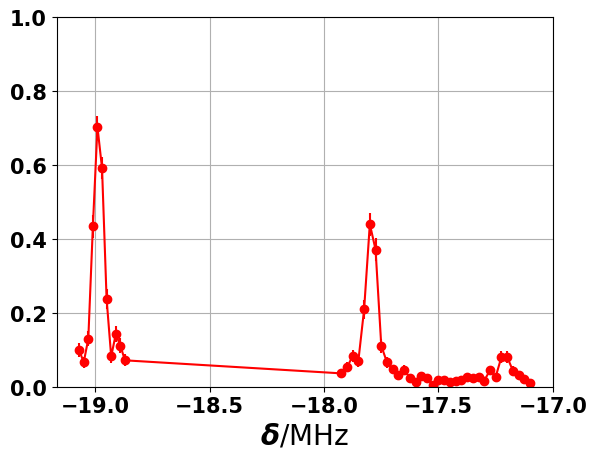
\includegraphics[width=4.5cm]{../../experiments/misc/imgs/data_20170319_213303_r3_before.png}
    }
  \end{columns}
\end{frame}

\begin{frame}{Cooling sequence}
  \begin{tikzpicture}
    \draw[line width=1] (0, 0) node[fill=green!20,draw,rounded corners,align=center]
    {
      Axial: $8$th\\
      Axial: $7$th\\
      Radial A: $2$nd\\
      Axial: $8$th\\
      Axial: $7$th\\
      Radial B: $2$nd} --
    ++(2.7, 0) node[fill=green!20,draw,rounded corners,align=center]
    {
      Axial: $7$th\\
      Axial: $6$th\\
      Radial A: $2$nd\\
      Axial: $7$th\\
      Axial: $6$th\\
      Radial B: $2$nd};
    \path (5.4, 0) node[align=center] {$\cdots$};
    \draw[line width=1] (8.1, 0) node[fill=green!20,draw,rounded corners,align=center]
    {
      Axial: $2$nd\\
      Axial: $1$st\\
      Radial A: $1$st\\
      Axial: $2$nd\\
      Axial: $1$st\\
      Radial B: $1$st};
    \path (0, -1.7) node[rounded corners,align=center]
    {
      \LARGE $\mathbf{\times 8}$
    } --
    ++(2.7, 0) node[rounded corners,align=center]
    {
      \LARGE $\mathbf{\times 8}$
    } --
    ++(5.4, 0) node[rounded corners,align=center]
    {
      \LARGE $\mathbf{\times 20}$
    };
  \end{tikzpicture}
\end{frame}

\begin{frame}{Status}
  \begin{columns}
    \column{5cm}
    \begin{itemize}
    \item Radial-only cooling
    \item<2-> Axial-only cooling
    \item<3-> 3D cooling\\
      (Survival: $\approx 89\%$)
    \end{itemize}
    \vspace{0.5cm}
    \visible<3>{
      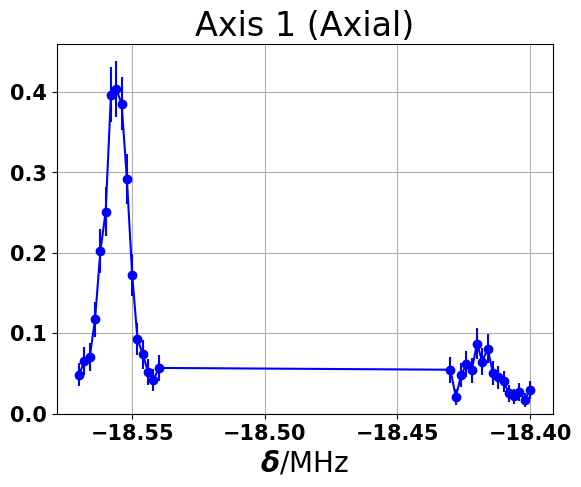
\includegraphics[width=5cm]{../../experiments/misc/imgs/data_20170324_010638_a1.png}
    }
    \column{6cm}
    \begin{center}
      \vspace{-1cm}
      \begin{tikzpicture}
        \visible<1>{
          \path (0, 0) node[align=center] {
            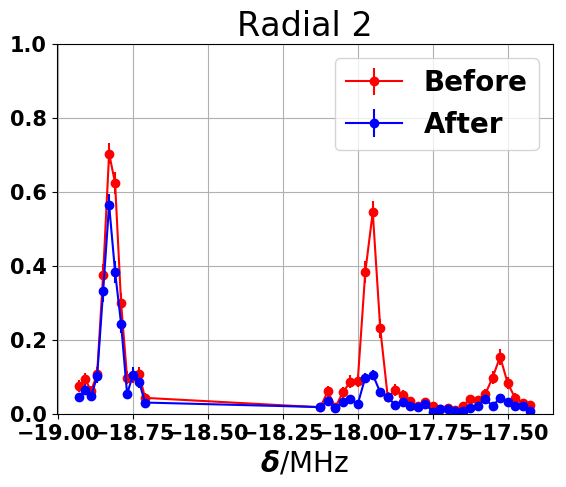
\includegraphics[width=4.5cm]{../../experiments/misc/imgs/data_20170319_213303_r2.png}\\
            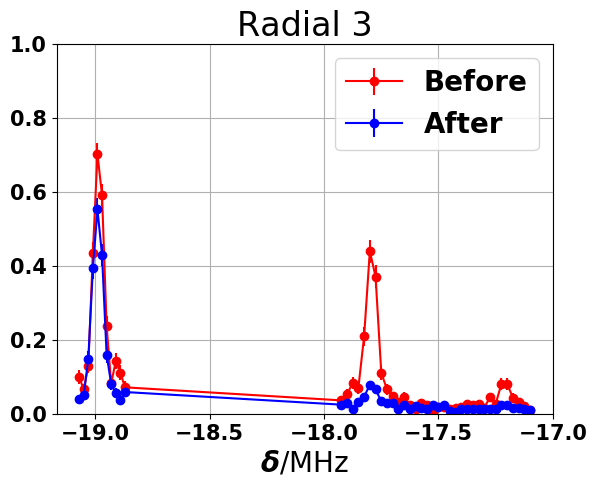
\includegraphics[width=4.5cm]{../../experiments/misc/imgs/data_20170319_213303_r3.png}
          };
        }
        \visible<2>{
          \path (0, 0) node[align=center] {
            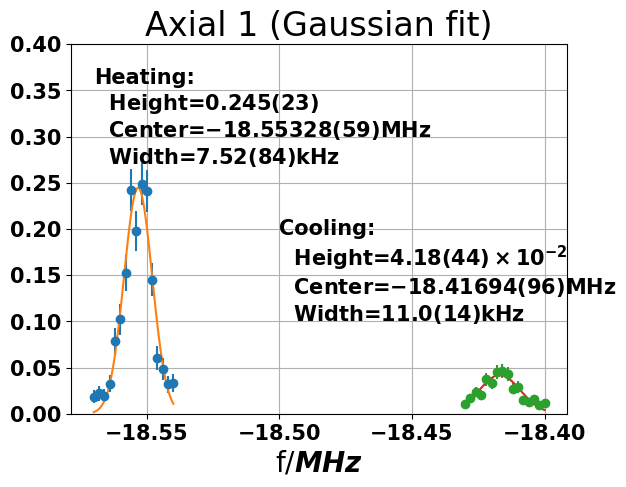
\includegraphics[width=6cm]{../../experiments/misc/imgs/data_20170313_220435_a1_fit.png}
          };
        }
        \visible<3>{
          \path (0, 0) node[align=center] {
            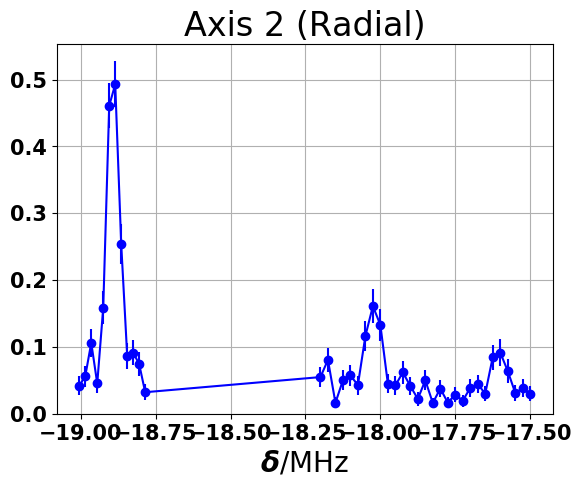
\includegraphics[width=5cm]{../../experiments/misc/imgs/data_20170324_010638_r2.png}\\
            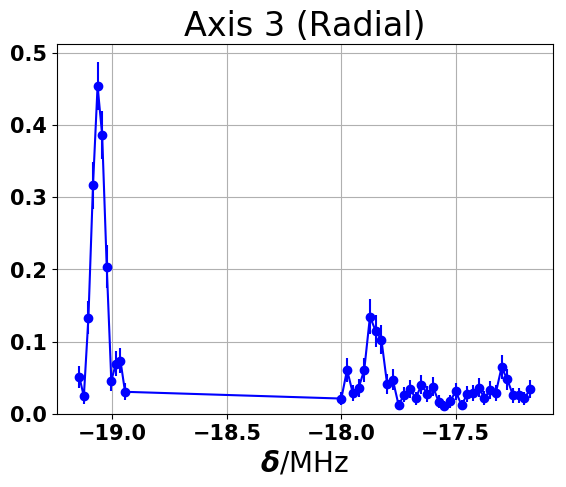
\includegraphics[width=5cm]{../../experiments/misc/imgs/data_20170324_010638_r3.png}
          };
        }
      \end{tikzpicture}
    \end{center}
  \end{columns}
\end{frame}

\begin{frame}{}
\end{frame}

\begin{frame}{Axial matrix element}
  \begin{center}
    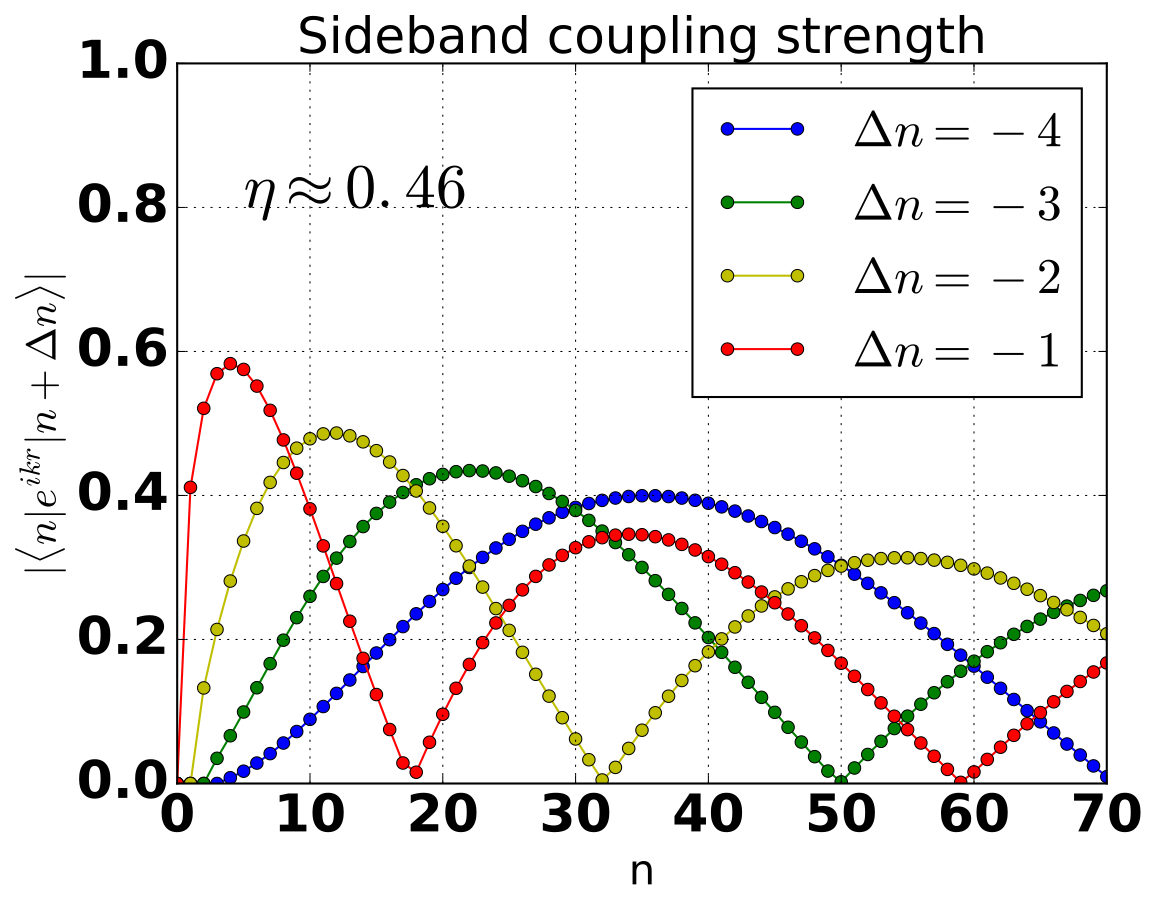
\includegraphics[width=5cm]{../../calculations/sideband_strength/imgs/coupling.png}
    \includegraphics[width=6.5cm]{{../../calculations/sideband_strength/imgs/coupling_0.46_0-6}.png}
  \end{center}
\end{frame}

\begin{frame}{Radial matrix element}
  \begin{center}
    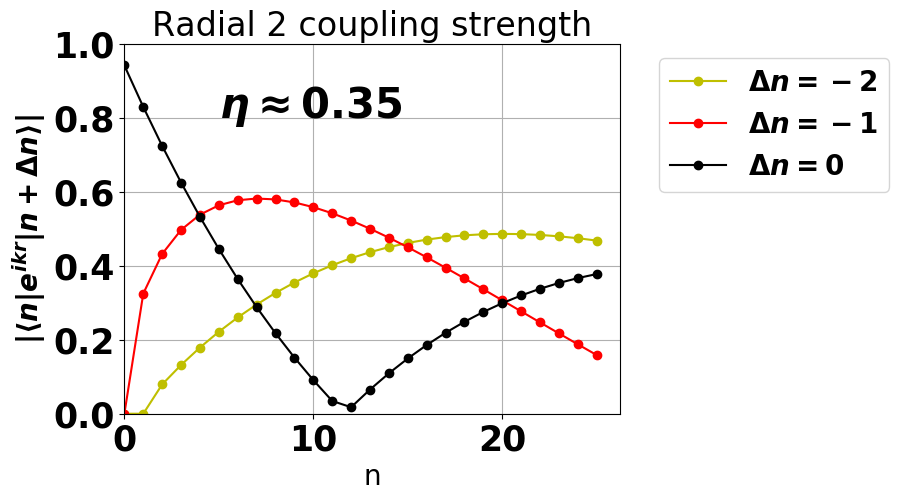
\includegraphics[width=6.5cm]{{../../calculations/sideband_strength/imgs/coupling_0.35_0-2}.png}
  \end{center}
\end{frame}

\end{document}
